\section{Lecture 5: The Fourier Transform}

Many signals are aperiodic, i.e. the time period $T \rightarrow\infty$. Such
signals cannot be treated by the Fourier series since this results in
$\omega_0\rightarrow 0$. Consequently, our sum over sinusoids of increasing
frequency makes no sense. Rather, we need to exchange the summations for
integrations over an infinitesimal in frequency,
%
\begin{displaymath}
  x(t) = \sum_{k=-\infty}^\infty a_k\ex{\im k\omega_0 t} \xrightarrow[T\rightarrow\infty]{}
  \int\dx{\omega} \ex{\im\omega t} \times \mathrm{something} \,.
\end{displaymath}
%
\begin{figure}[!htb]
  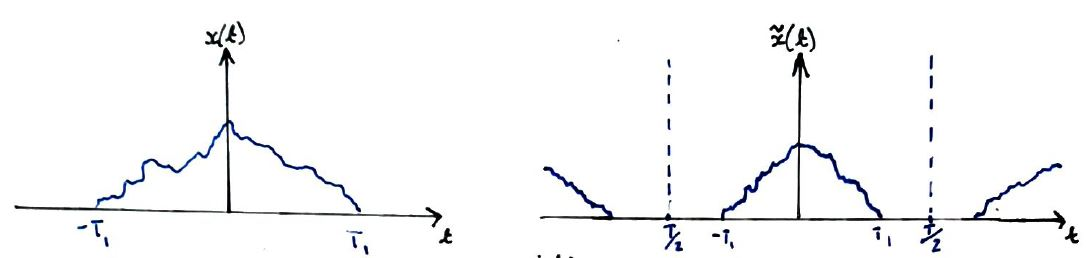
\includegraphics[width=\textwidth]{images/lecture_5_enforce_periodicity.JPG}
  \caption{
    An aperiodic signal (left) and its periodic form (right) where the time period
    has been chosen to include some time during which the signal is zero.
  }
  \label{fig::lecture_5_enforce_periodicity}
\end{figure}
%
Consider the aperiodic signal in Figure \ref{fig::lecture_5_enforce_periodicity}. We can force its periodicity (with
period $T$) by duplicating it. We'll refer to this
signal with ``enforced periodicity'' as $\tilde{x}(t)$, its Fourier synthesis
being
%
\begin{displaymath}
  \tilde{x}(t) = \sum_{k=-\infty}^\infty a_k\ex{\im k\omega_0 t} \,,
\end{displaymath}
%
and Fourier analysis
%
\begin{displaymath}
  a_k = \frac{1}{T}\int_{-T/2}^{T/2} \dx{t} \tilde{x}(t)\ex{-\im k\omega_0 t} \,.
\end{displaymath}
%
However, on the domain $t\in[-\frac{T}{2},\frac{T}{2}]$, $\tilde{x}(t)$ is simply $x(t)$.
And since this signal has no duplicates, the integral can be evaluated indefinitely
%
\begin{displaymath}
  a_k = \frac{1}{T}\int \dx{t} x(t)\ex{-\im k\omega_0 t} \,.
\end{displaymath}
%
Now, defining the \textbf{Fourier Transform} as
%
\begin{equation}
  X(\omega) = \int \dx{t} x(t)\ex{-\im\omega t} \,,
\end{equation}
%
we can formulate the Fourier coefficients
%
\begin{displaymath}
  a_k = \frac{1}{T} X(k\omega_0) \,,
\end{displaymath}
%
presenting us with the expression
%
\begin{displaymath}
  \tilde{x}(t) = \frac{1}{T}\sum_{k=-\infty}^\infty X(k\omega_0)\ex{\im k\omega_0 t} \,.
\end{displaymath}
%
Taking advantage of the fact that $\omega_0 = \frac{2\pi}{T}$,
%
\begin{displaymath}
  \tilde{x}(t) = \frac{1}{2\pi}\sum_{k=-\infty}^\infty \left[X(k\omega_0)\ex{\im k\omega_0 t}\right]\omega_0 \,.
\end{displaymath}
%
The above form allows us to gain some insight into this Fourier synthesis.
Take the example in Figure \ref{fig::lecture_5_riemann}. We see that the summation in our expression for
$\tilde{x}(t)$ is the Riemann sum, and
%
\begin{displaymath}
  \lim_{\omega_0\rightarrow 0}\tilde{x}(t) = x(t) \,.
\end{displaymath}
%
\begin{figure}[!htb]
  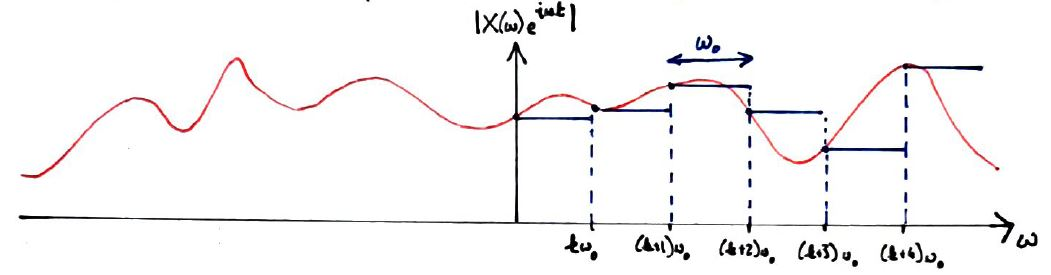
\includegraphics[width=\textwidth]{images/lecture_5_riemann.JPG}
  \caption{
    The value of the periodic signal $\tilde{x}(t)$ at time $t$ is given by the Riemann
    sum of Fourier coefficients multiplied by complex exponentials. The sum is built up
    from rectangles of width $\omega_0$ along the frequency axis. Note that the absolute
    values of the Fourier coefficients are plotted since these are complex-valued quantities.
  }
  \label{fig::lecture_5_riemann}
\end{figure}
%
Since this limit coincides with $T\rightarrow\infty$, we are effectively
pushing the duplicate copies of $x(t)$ infinitely far away, and
%
\begin{displaymath}
  \lim_{\omega\rightarrow 0}\frac{\omega_0}{2\pi}\sum_{k=-\infty}^\infty \ex{\im k\omega_0 t}
  = \frac{1}{2\pi}\int\dx{\omega}X(\omega)\ex{\im\omega t} \,.
\end{displaymath}
%
We're finally left with a pair of expressions that are the continuous-time
analogues of the Fourier synthesis and analysis:
%
\begin{align}
  x(t) &= \frac{1}{2\pi}\int\dx{\omega} X(\omega)\ex{\im\omega t} \\
  X(\omega) &= \int\dx{t} x(t)\ex{-\im\omega t} \,,
\end{align}
%
the former being the \textbf{Inverse Fourier Transform} and the latter being
the \textbf{Fourier Transform}.

\subsection{Validity of the Fourier Transform}
%
We have a similar set of criteria to those of the Fourier series regarding
the types of signals that are viable candidiates for the Fourier transform:
%
\begin{enumerate}
\item $x(t)$ must be square-integrable, i.e. $\int|x(t)|^2 < \infty$.
\item The signal must contain a finite number of extrema.
\item The signal must contain a finite number of discontinuities.
\end{enumerate}

\subsection{Some Fourier Transform Identities}
%
\begin{enumerate}
\item For the delta function, i.e. $x(t) = \delta(t)$, the Fourier transform is
  given by
  %
  \begin{displaymath}
    X(\omega) = \int \dx{t} \delta(t)\ex{-\im\omega t} = \ex{-\im\omega\times 0} = 1 \,,
  \end{displaymath}
  %
  i.e. a constant for all frequencies.
\item For the shifted delta function, i.e. $x(t) = \delta(t-t_0)$, the Fourier transform
  is given by
  %
  \begin{displaymath}
    X(\omega) = \int \dx{t} \delta(t-t_0)\ex{-\im\omega t} = \ex{-\im\omega t_0} \,.
  \end{displaymath}
  %
  These coefficients all have the same magnitude, $\sqrt{\ex{-\im\omega t_0}\ex{\im\omega t_0}} = 1$,
  but rotated on the unit circle in the complex plane, and so all have different phase.
\item For the sum of delta functions $x(t) = \delta(t-t_0) + \delta(t+t_0)$,
  %
  \begin{displaymath}
    X(\omega) = \ex{-\im\omega t_0} + \ex{-\im\omega t_0} = 2\cos(\omega t_0) \,.
  \end{displaymath}
\item For the decaying step function, $x(t) = \ex{-at}u(t)$, where $a > 0$,
  %
  \begin{align*}
    X(\omega) &= \int \dx{t} \ex{-at}u(t)\ex{-\im\omega t} = \int_0^\infty\dx{t} \ex{-t(\im\omega + a)} \\
    &= \left.-\frac{1}{(\im\omega + a)} \ex{-t(\im\omega + a)}\right|_0^\infty = \frac{1}{\im\omega + a} \,.
  \end{align*}
\item For the ``top hat'' function which is high on the domain $[-T/2,T/2]$
  %
  \begin{align*}
    X(\omega) &= \int_{-T/2}^{T/2}\dx{t}x(t)\ex{-\im\omega t} = \int_{-T/2}^{T/2}\dx{t}\ex{-\im\omega t} \\
    &= \left.-\frac{1}{\im\omega} \ex{-\im\omega t}\right|_{-T/2}^{T/2} = \frac{1}{\im\omega}
    \left(\ex{\im\omega\frac{T}{2}} - \ex{-\im\omega\frac{T}{2}}\right) \\
    &= \frac{2}{\omega}\sin\left(\omega\frac{T}{2}\right) = T\sinc\left(\frac{\omega T}{2}\right) \,.
  \end{align*}
\item For a ``top hat'' in the frequency domain which is high on the domain $[-\omega_0/2,\omega_0/2]$
  %
  \begin{align*}
    x(t) &= \frac{1}{2\pi}\int \dx{\omega}X(\omega)\ex{\im\omega t}
    = \frac{1}{2\pi}\int_{-\omega_0/2}^{\omega_0/2} \dx{\omega} \ex{\im\omega t} \\
    &= \left. \frac{1}{2\pi\im t} \ex{\im\omega t}\right|_{-\omega_0/2}^{\omega_0/2}
    = \frac{1}{2\pi\im t} \left(\ex{\im\frac{\omega_0}{2}t} - \ex{-\im\frac{\omega_0}{2}t}\right) \\
    &= \frac{\omega_0}{2\pi}\sinc\left(\frac{\omega_0}{2}t\right) \,.
  \end{align*}
  %
  This result demonstrates the duality of Fourier transform pairs -- a top hat in the
  time domain becomes a $\sinc$ in the frequency domain, and \textit{vice versa}. Similarly,
  a delta function in the time domain becomes a constant in the frequency domain and
  \textit{vice versa}.
\end{enumerate}
%
If $x(t)$ is periodic, then we can choose to use either the Fourier series or Fourier
transform. Let's choose an impulse train, $x(t) = \sum_{k=-\infty}^\infty\delta(t - kT)$,
a series of delta functions that are $T$ apart. Using the Fourier series,
%
\begin{displaymath}
  a_k = \frac{1}{T}\int_{-T/2}^{T/2}\dx{t} x(t)\ex{-\im k\frac{2\pi}{T}t} = \frac{1}{T} \,,
\end{displaymath}
%
as we have seen before since over the interval $[-T/2,T/2]$, the only non-zero point is
at $t=0$.

Suppose $x(t)$ is periodic, and consequently can be represented as a Fourier synthesis.
Then, from the Fourier transform, we have that
%
\begin{displaymath}
  X(\omega) = \int\dx{t}x(t)\ex{-\im\omega t}
  = \sum_{k=-\infty}^\infty\int\dx{t}a_k\ex{\im k\omega_0 t}\ex{-\im\omega t}
  = \sum_{k=-\infty}^\infty \int\dx{t}a_k\ex{\im (k\omega_0 - \omega) t} \,.
\end{displaymath}
%
The integral in this final expression can be simplified through use of the identity
%
\begin{displaymath}
  \int\dx{t}\ex{i(\omega - \omega_0)t} = 2\pi\delta(\omega - \omega_0) \,.
\end{displaymath}
%
This can be proven through use of a test function $G(\omega)$,
%
\begin{displaymath}
  \frac{1}{2\pi}\int\dx{\omega} G(\omega)\left(
    \int\dx{t}\ex{\im(\omega-\omega_0)t}
  \right)  = \int\dx{t}\ex{-\im\omega_0 t} \frac{1}{2\pi}\int\dx{\omega} G(\omega)\ex{\im\omega t} \,.
\end{displaymath}
%
But this second integral is simply the inverse Fourier transform of $G(\omega)$,
%
\begin{displaymath}
  \int\dx{t}\ex{-\im\omega_0 t} g(t) = G(\omega_0) \,,
\end{displaymath}
%
which is subsequently Fourier transformed, and we see that the entire operation
has simply changed the frequency variable from $\omega$ to $\omega_0$, as if
we have selected for $\omega_0$ with a delta function. Consequently, returning to
our expression for $X(\omega)$,
%
\begin{displaymath}
  X(\omega) = \sum_{k=-\infty}^\infty \int\dx{t}a_k\ex{\im (k\omega_0 - \omega) t}
  = \sum_{k=-\infty}^\infty 2\pi a_k \delta(\omega - k\omega_0) \,,
\end{displaymath}
%
where we've taken advantage of the fact that $\delta(x) = \delta(-x)$ (think about
this like a Kronecker delta: $\delta_{i,j} = \delta_{-i,-j}$). Our final form for
$X(\omega)$ lends itself to being graphed -- it's simply an infinite series of shifted
delta functions that are spaced by $\omega_0$, as can be see in Figure
\ref{fig::lecture_5_fourier_deltas}.
%
\begin{figure}[!htb]
  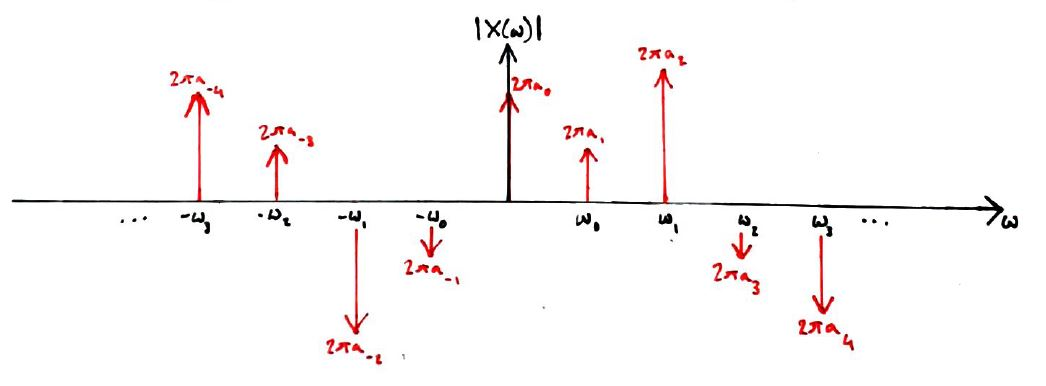
\includegraphics[width=\textwidth]{images/lecture_5_fourier_deltas.JPG}
  \caption{
    The Fourier transform of a periodic function is a series of shifted
    delta functions spaced by $\omega_0$ in the frequency domain, each one
    with magnitude $|2\pi a_k|$.
  }
  \label{fig::lecture_5_fourier_deltas}
\end{figure}

\begin{exmp}
  Consider the spectrum with $X(\pm\omega_0) = \pi$ and $X(\omega) = 0$
  for all other values of $\omega$. Conseqeuntly, we have
  %
  \begin{displaymath}
    x(t) = \frac{1}{2\pi}\int\dx{\omega}X(\omega)\ex{\im\omega t}
    = \frac{1}{2\pi} \int\dx{\omega}\delta(\omega\pm\omega_0)\ex{\im\omega t}
    = \frac{1}{2\pi}\left[\pi\ex{\im\omega_0 t} + \pi\ex{-\im\omega_0 t}\right]
    = \cos(\omega_0 t) \,,
  \end{displaymath}
  %
  which satisfies our condition of $a_k = a_{-k}$ for real-valued signals.
\end{exmp}

\subsection{Properties of the Fourier Transform}
%
\begin{enumerate}
\item (\textbf{Linearity}) Given the Fourier pairs $x(t) \Longleftrightarrow X(\omega)$ and
  $y(t) \Longleftrightarrow Y(\omega)$, then
  %
  \begin{displaymath}
    \alpha x(t) + \beta y(t) \Longleftrightarrow \alpha X(\omega) + \beta Y(\omega) \,.
  \end{displaymath}
  %
\item (\textbf{Time Shifting}) Time-shifting results in a phase change in the
  spectral coefficients, $x(t-t_0) \Longleftrightarrow X(\omega)\ex{-\im\omega t_0}$.
\item (\textbf{Real Signals}) If $x(t)$ is real, then $\Re(X(\omega)) = \Re(X(-\omega))$
  and $\Im(X(\omega)) = -\Im(X(-\omega))$, i.e. the real part is even and the imaginary
  part is odd. Together, this implies Hermitian symmetry, $X(\omega) = X(-\omega)^*$.
\item (\textbf{Even and Odd Signals}) For real $x(t)$,
  $\mathrm{Even}(x(t)) \Longleftrightarrow \Re(X(\omega))$ and
  $\mathrm{Odd}(x(t)) \Longleftrightarrow \im\Im(X(\omega))$.
\item (\textbf{Differentiability})
  %
  \begin{displaymath}
    x^\prime(t) \Longleftrightarrow \im\omega X(\omega) \,,
  \end{displaymath}
  %
  \begin{displaymath}
    \int_{-\infty}^t \dx{\tau}x(\tau) \Longleftrightarrow \frac{1}{\im\omega}X(\omega) + \pi X(0)\delta(\omega) \,.
  \end{displaymath}
\item (\textbf{Scaling}) Consider $x(t) \Longleftrightarrow X(\omega)$. Then,
  %
  \begin{displaymath}
    x(at) = \frac{1}{|a|} X\left(\frac{\omega}{a}\right) \,.
  \end{displaymath}
  %
  If $a$ is large, then $x(at)$ is squeezed and $\frac{1}{|a|} X\left(\frac{\omega}{a}\right)$
  is stretched. Conversely, if $a$ is small then the opposite happens.
\end{enumerate}

\subsection{Analytic Signals}
%
Many signals of interest are real-valued; owing to the Hermitian symmetry
of the spectrums of these signals, the negative frequencies are superfluous
since $Z(\omega) = Z(-\omega)^*$, and as a result hold no additional
information. An \textbf{analytic signal} is a signal with no negative
frequency components in its spectrum, and consequently can be writen
%
\begin{displaymath}
  z(t) = \frac{1}{2\pi}\int_0^\infty \dx{\omega}Z(\omega)\ex{\im\omega t} \,,
\end{displaymath}
%
which facilitates some mathematical manipulations. This (complex) analytic
signal can be generated through use of the \textbf{Hilbert Transform}, which
shifts the phase of positive frequencies by $-\pi/2$ and the phase of negative
frequencies by $\pi/2$ (QQ: Add something on Hilbert Transform). Then, the
analytic signal is constructed from the real signal $x(t)$ and its Hilbert
Transform $y(t) = \mathcal{H}[y(t)]$, i.e. $z(t) = x(t) + \im y(t)$.\\
%
To see why this works, consider the positive and negative frequency
components of $x(t)$ at some frequency $\omega_0$,
%
\begin{displaymath}
  x_+(t) = \ex{\im\omega_0 t} \quad\mathrm{and}\quad x_-(t) = \ex{-\im\omega_0 t} \,.
\end{displaymath}
%
Performing the Hilbert transform on these two functions,
%
\begin{displaymath}
  \mathcal{H}[x_+(t)] = y_+(t) = \ex{\im\omega_0 t}\ex{-\im\pi/2} = -\im\ex{\im\omega_0 t}
  \quad\mathrm{and}\quad
  \mathcal{H}[x_-(t)] = y_-(t) = \ex{-\im\omega_0 t}\ex{\im\pi/2} = \im\ex{-\im\omega_0 t} \,.
\end{displaymath}
%
Now, constructing the analytic signal,
%
\begin{align*}
  z_+(t) &= x_+(t) + \im y_+(t) = \ex{\im\omega_0 t} - \im^2\ex{\im\omega_0 t} = 2\ex{\im\omega_0 t} \\
  z_-(t) &= x_-(t) + \im y_-(t) = \ex{-\im\omega_0 t} + \im^2\ex{\im\omega_0 t} = 0 \,,
\end{align*}
%
and we see that the negative frequency component has been filtered out while
the positive frequency component has a gain of $2$. As such,
%
\begin{displaymath}
  Z(\omega) = 2H(\omega)X(\omega) = \left\{\begin{array}{ccl}
      2X(\omega) & & \omega > 0 \\
      X(\omega) & & \omega = 0 \\
      0 & & \omega < 0
    \end{array}\right.\,,
\end{displaymath}
%
where $H(\omega)$ is the Heaviside function.
%
\begin{exmp}
  Consider the real signal $x(t) = \cos(\omega_0 t)$. The Hilbert transform of this
  is
  %
  \begin{displaymath}
    \mathcal{H}[x(t)]
    = \frac{1}{2}\left[\ex{\im\omega_0 t}\ex{-\im\pi/2} + \ex{-\im\omega_0 t}\ex{\im\pi/2}\right]
    = \frac{1}{2}\left[\im\ex{-\im\omega_0 t} - \im\ex{\im\omega_0 t}\right]
    = \sin(\omega_0 t) \,.
  \end{displaymath}
  %
  Then, the analytic signal is
  %
  \begin{displaymath}
    z(t) = \cos(\omega_0 t) + \im\sin(\omega_0 t) = \ex{\im\omega_0 t}
  \end{displaymath}
  %
  In the frequency domain, $X(\omega)$ has impulses at $\pm\omega_0$ with amplitudes
  $1/2$. For the Hilbert transform, we see that $Y(\omega)$ has an impulses
  at $\omega_0$ and $-\omega_0$ with amplitudes $-\im/2$ and $\im/2$, respectively. 
  In constructing the analytic signal, $\im Y(\omega)$ has impulses again at $\omega_0$
  and $-\omega_0$ but now with amplitudes $1/2$ and $-1/2$, respectively. Finally,
  the analytic signal $Z(\omega) = X(\omega) + \im Y(\omega)$ has a single unit impulse
  at $\omega_0$.
\end{exmp}
%
\begin{exmp}
  A motivating example for the use of analytic signals is some slowly-varying
  amplitude envelope, $A(t)$, which is mixed with some carrier signal $\cos(\omega_c t)$,
  where $\omega_c$ is of higher frequency than any of the components of $A(t)$.
  Assume $A(t)$ is a single low-frequency tone $A(t) = \cos(\omega_a t)$.
  Then, we have $x(t) = A(t)\cos(\omega_c t) = \cos(\omega_c t)\cos(\omega_a t)$;
  this is nothing more than amplitude modulation -- on a radio, one tunes into
  the carrier frequency and $A(t)$ is the associated information content. Our
  mixed signal is then
  %
  \begin{displaymath}
    x(t) = \frac{1}{4}\left(
    \ex{\im(\omega_c + \omega_a)t} + \ex{\im(\omega_c - \omega_a)t} +
    \ex{\im(-\omega_c + \omega_a)t} + \ex{\im(-\omega_c - \omega_a)t}
    \right) \,.
  \end{displaymath}
  %
  Recalling that $\omega_c > \omega_a$, we can identify the positive frequencies as
  $\omega_c \pm \omega_a$ while the negative frequencies are at $-\omega_c \pm\omega_a$. The
  Hilbert transforms are then
  %
  \begin{displaymath}
    y_+(t) = -\frac{\im}{4}\left(\ex{\im(\omega_c + \omega_a)t} + \ex{\im(\omega_c - \omega_a)t}\right) 
    \quad\mathrm{and}\quad
    y_-(t) = \frac{\im}{4}\left(\ex{\im(-\omega_c + \omega_a)t} + \ex{\im(-\omega_c - \omega_a)t}\right) \,,
  \end{displaymath}
  %
  such that
  %
  \begin{align*}
    y(t) &= \frac{1}{4\im}\left(
    \color{red}{\ex{\im(\omega_c + \omega_a)t}} \color{blue}{+ \ex{\im(\omega_c - \omega_a)t}}
    \color{blue}{-\ex{\im(-\omega_c + \omega_a)t}} \color{red}{- \ex{\im(-\omega_c - \omega_a)t}} 
    \right) \\
    &= \frac{1}{2}\left(
    \color{red}{\sin((\omega_c + \omega_a)t)} \color{blue}{+ \sin((\omega_c - \omega_a)t)}\right)
    = \sin(\omega_c t)\cos(\omega_a t) = A(t)\sin(\omega_c t) \,.
  \end{align*}
  %
  The analytic signal is then simply
  $z(t) = A(t)\left[\cos(\omega_c t) + \im\sin(\omega_c t)\right] = A(t)\ex{\im\omega_c t}$.
  Amplitude demodulation involves nothing more than taking the magnitude of $z(t)$.
\end{exmp}

\subsection{The Short-Time Fourier Transform}
%
The scaling property leads us to a rather profoud result, since it suggests
a tradeoff between our ability to simultaneously ``concentrate'' both a
function and its Fourier transform in their respective domains. This is a
result that is one of the bedrocks of quantum theory, where position and
momentum are Fourier transform pairs (to within Planck's constant), and
manifests itself as the famous Heisenberg Uncertainty Principle, where
once cannot simultaneously know both the position and momentum of a particle
to arbitrary precision. Knowledge about the particle's position to infinite
accuracy results in a complete loss of knowledge about the particle's
momentum, and \textit{vice versa}. We see that this property is the same for
the generic Fourier transform pairs we've considered in this chapter -- the
Fourier transform of a delta function is a constant across all frequency,
and \textit{vice versa}.
%
The complete derivation of the \textbf{Gabor Limit}, the maximum resolution
with which both time and frequency can be quantified in signal processing,
is presented in Section 3.11 of Brad Osgood's lecture notes on
``The Fourier Transform and its Applications'', to which the reader is
re-directed. We simply present the final result here,
%
\begin{equation}
  \sigma_t\cdot\sigma_\omega \geq \frac{1}{4\pi} \approx \textrm{0.08\;Cycles} \,,
\end{equation}
%
where $\sigma_t, \sigma_\omega$ are the standard deviations in the time and
frequency domains, respectively.

This Gabor limit presents us with an opportunity in signal processing. For a
complex time domain signal, different frequencies appear at different times.
Consider the example of playing an instrument -- in a simplistic sense,
this is simply a sequence of notes, or discrete frequencies, in time. Yet, if
we take the Fourier transform of an audio recording of the piece, all we can
see is that these discrete frequencies were present in the time-domain signal,
it tells us nothing about when in the piece the frequencies were active. In
effect, we're presented with either an infinite precision in the time domain
(the audio track) or an infinite precision in the frequency domain (the
Fourier transform). And this is where the Gabor limit becomes important -- in
principle, I can work out a little bit about both, as long as the product
of standard deviations in time and frequency do not exceed $\frac{1}{4\pi}$.\\

One method for generating a \textbf{spectrogram}, a plot of time against
frequency upon which magnitudes are plotted (i.e. how ``active'' a certain
frequency is at a certain point in time) is the is the
\textbf{Short-Time Fourier Transform} (STFT). 
